\documentclass[12pt]{report}
\usepackage{amsmath}
\usepackage{latexsym}
\usepackage{amsfonts}
\usepackage[normalem]{ulem}
\usepackage{soul}
\usepackage{array}
\usepackage{amssymb}
\usepackage{extarrows}
\usepackage{graphicx}
\usepackage[backend=biber,
style=numeric,
sorting=none,
isbn=false,
doi=false,
url=false,
]{biblatex}\addbibresource{bibliography-biblatex.bib}

\usepackage{subfig}
\usepackage{wrapfig}
\usepackage{wasysym}
\usepackage{enumitem}
\usepackage{adjustbox}
\usepackage{ragged2e}
\usepackage[svgnames,table]{xcolor}
\usepackage{tikz}
\usepackage{longtable}
\usepackage{changepage}
\usepackage{setspace}
\usepackage{hhline}
\usepackage{multicol}
\usepackage{tabto}
\usepackage{float}
\usepackage{multirow}
\usepackage{makecell}
\usepackage{fancyhdr}
\usepackage[toc,page]{appendix}
\usepackage[hidelinks]{hyperref}
\usetikzlibrary{shapes.symbols,shapes.geometric,shadows,arrows.meta}
\tikzset{>={Latex[width=1.5mm,length=2mm]}}
\usepackage{flowchart}\usepackage[paperheight=11.69in,paperwidth=8.27in,left=1.0in,right=1.0in,top=1.5in,bottom=1.5in,headheight=1in]{geometry}
\usepackage[utf8]{inputenc}
\usepackage[T1]{fontenc}
\usepackage[spanish]{babel}
\TabPositions{0.5in,1.0in,1.5in,2.0in,2.5in,3.0in,3.5in,4.0in,4.5in,5.0in,5.5in,6.0in,}

\urlstyle{same}

\renewcommand{\_}{\kern-1.5pt\textunderscore\kern-1.5pt}

 %%%%%%%%%%%%  Set Depths for Sections  %%%%%%%%%%%%%%

% 1) Section
% 1.1) SubSection
% 1.1.1) SubSubSection
% 1.1.1.1) Paragraph
% 1.1.1.1.1) Subparagraph


\setcounter{tocdepth}{5}
\setcounter{secnumdepth}{5}


 %%%%%%%%%%%%  Set Depths for Nested Lists created by \begin{enumerate}  %%%%%%%%%%%%%%


\setlistdepth{9}
\renewlist{enumerate}{enumerate}{9}
		\setlist[enumerate,1]{label=\arabic*)}
		\setlist[enumerate,2]{label=\alph*)}
		\setlist[enumerate,3]{label=(\roman*)}
		\setlist[enumerate,4]{label=(\arabic*)}
		\setlist[enumerate,5]{label=(\Alph*)}
		\setlist[enumerate,6]{label=(\Roman*)}
		\setlist[enumerate,7]{label=\arabic*}
		\setlist[enumerate,8]{label=\alph*}
		\setlist[enumerate,9]{label=\roman*}

\renewlist{itemize}{itemize}{9}
		\setlist[itemize]{label=$\cdot$}
		\setlist[itemize,1]{label=\textbullet}
		\setlist[itemize,2]{label=$\circ$}
		\setlist[itemize,3]{label=$\ast$}
		\setlist[itemize,4]{label=$\dagger$}
		\setlist[itemize,5]{label=$\triangleright$}
		\setlist[itemize,6]{label=$\bigstar$}
		\setlist[itemize,7]{label=$\blacklozenge$}
		\setlist[itemize,8]{label=$\prime$}



 %%%%%%%%%%%%  Header here  %%%%%%%%%%%%%%


\pagestyle{fancy}
\fancyhf{}
\lhead{ 
\vspace{\baselineskip}
}
\lfoot{ 
\vspace{\baselineskip}
}
\renewcommand{\headrulewidth}{0pt}
\setlength{\topsep}{0pt}\setlength{\parindent}{0pt}

 %%%%%%%%%%%%  This sets linespacing (verticle gap between Lines) Default=1 %%%%%%%%%%%%%%


\renewcommand{\arraystretch}{1.3}


\date{}


%%%%%%%%%%%%%%%%%%%% Document code starts here %%%%%%%%%%%%%%%%%%%%



\begin{document}




%%%%%%%%%%%%%%%%%%%% Figure/Image No: 1 starts here %%%%%%%%%%%%%%%%%%%%

\begin{figure}[H]
	\begin{Center}
		
\includegraphics[width=2.01in,height=1.69in]{./media/image7.png}
	\end{Center}
\end{figure}


%%%%%%%%%%%%%%%%%%%% Figure/Image No: 1 Ends here %%%%%%%%%%%%%%%%%%%%

\setlength{\parskip}{12.0pt}
\begin{Center}
\textbf{\   }
\end{Center}
\begin{Center}
\textbf{FACULTAD DE INGENIERÍA}
\end{Center}
\begin{Center}
\textbf{INGENIERÍA CIVIL INFORMÁTICA}
\end{Center}
\begin{Center}
{\fontsize{20pt}{24.0pt}\selectfont  }
\end{Center}

\vspace{\baselineskip}
 {\fontsize{20pt}{24.0pt}\selectfont \textbf{\uline{ }}}
\begin{Center}
{\fontsize{20pt}{24.0pt}\selectfont \textbf{\uline{Ciencia de Datos}}}
\end{Center}

\vspace{\baselineskip}
\begin{Center}
{\fontsize{20pt}{24.0pt}\selectfont \textbf{\uline{Análisis y Preprocesamiento}}}
\end{Center}
\begin{Center}
{\fontsize{20pt}{24.0pt}\selectfont \textbf{\uline{\url{https://github.com/JavierTallarin/proyecto-CreditoBancario-Ciencia-De-Datos}}}}
\end{Center}
 
 
 
\begin{Center}
 \textbf{Jorge Ahumada Margarit}
\end{Center}
\begin{Center}
\textbf{Javier Bravo Orellana}
\end{Center}
\begin{Center}
\textbf{Cristóbal Olave Herrera}
\end{Center}
\begin{Center}
\textbf{Luis Rodriguez Zamora}
\end{Center}

\vspace{\baselineskip}


\vspace{\baselineskip}

\vspace{\baselineskip}

\vspace{\baselineskip}

\vspace{\baselineskip}

\vspace{\baselineskip}


 %%%%%%%%%%%%  This Produces Table Of Contents %%%%%%%%%%%%%%

\tableofcontents
\addcontentsline{toc}{chapter}{Contents}

\vspace{\baselineskip}

\vspace{\baselineskip}

\vspace{\baselineskip}

\vspace{\baselineskip}

\vspace{\baselineskip}

\vspace{\baselineskip}

\vspace{\baselineskip}

\vspace{\baselineskip}

\vspace{\baselineskip}

\vspace{\baselineskip}

\vspace{\baselineskip}

\vspace{\baselineskip}

\vspace{\baselineskip}

\vspace{\baselineskip}

\vspace{\baselineskip}

\vspace{\baselineskip}

\vspace{\baselineskip}
\vspace{\baselineskip}
\vspace{\baselineskip}
\vspace{\baselineskip}
\vspace{\baselineskip}
\vspace{\baselineskip}
\vspace{\baselineskip}
\vspace{\baselineskip}
\vspace{\baselineskip}
\vspace{\baselineskip}
\vspace{\baselineskip}
\vspace{\baselineskip}
\vspace{\baselineskip}
\vspace{\baselineskip}
\vspace{\baselineskip}

\vspace{\baselineskip}
\section{ Introducción}

\vspace{\baselineskip}
Este conjunto de datos de UCI contiene cantidad crediticia, datos demográficos, historial de pagos y extractos de facturas de clientes de tarjetas de crédito en Taiwán desde abril de 2005 hasta septiembre de 2005. Finalmente esta investigación tiene como objetivo el caso de los pagos por incumplimiento de los clientes en Taiwán.

\vspace{\baselineskip}

\vspace{\baselineskip}

\vspace{\baselineskip}

\vspace{\baselineskip}

\vspace{\baselineskip}

\vspace{\baselineskip}

\vspace{\baselineskip}

\vspace{\baselineskip}

\vspace{\baselineskip}

\vspace{\baselineskip}

\vspace{\baselineskip}

\vspace{\baselineskip}

\vspace{\baselineskip}

\vspace{\baselineskip}

\vspace{\baselineskip}

\vspace{\baselineskip}

\vspace{\baselineskip}

\vspace{\baselineskip}

\vspace{\baselineskip}

\vspace{\baselineskip}

\vspace{\baselineskip}

\vspace{\baselineskip}

\vspace{\baselineskip}

\vspace{\baselineskip}

\vspace{\baselineskip}

\vspace{\baselineskip}

\vspace{\baselineskip}

\vspace{\baselineskip}

\vspace{\baselineskip}

\vspace{\baselineskip}

\vspace{\baselineskip}

\vspace{\baselineskip}

\vspace{\baselineskip}

\vspace{\baselineskip}
\section{Objetivos}

\vspace{\baselineskip}

\vspace{\baselineskip}

\vspace{\baselineskip}
\begin{itemize}
	\item Realizar estadística descriptiva básica para conocer los datos que se encuentran en el dataset y cuáles son sus características.
	\item Reconocer patrones presentes en el dataset que nos servirán para clasificar posteriormente con la ayuda de modelos de predicción y clasificadores probabilísticos.
	\item Finalmente la finalidad de este trabajo investigativo es estimar la probabilidad de incumplimiento de los clientes de Taiwán, de esta manera se podrá decidir si se le asigna el crédito a algún cliente del banco.
\end{itemize}

\vspace{\baselineskip}

\vspace{\baselineskip}

\vspace{\baselineskip}

\vspace{\baselineskip}

\vspace{\baselineskip}

\vspace{\baselineskip}

\vspace{\baselineskip}

\vspace{\baselineskip}

\vspace{\baselineskip}

\vspace{\baselineskip}

\vspace{\baselineskip}

\vspace{\baselineskip}

\vspace{\baselineskip}

\vspace{\baselineskip}

\vspace{\baselineskip}

\vspace{\baselineskip}

\vspace{\baselineskip}

\vspace{\baselineskip}

\vspace{\baselineskip}

\vspace{\baselineskip}

\vspace{\baselineskip}

\vspace{\baselineskip}

\vspace{\baselineskip}

\vspace{\baselineskip}

\vspace{\baselineskip}

\vspace{\baselineskip}

\vspace{\baselineskip}

\vspace{\baselineskip}

\vspace{\baselineskip}

\vspace{\baselineskip}

\vspace{\baselineskip}

\vspace{\baselineskip}

\vspace{\baselineskip}

\vspace{\baselineskip}

\vspace{\baselineskip}

\vspace{\baselineskip}

\vspace{\baselineskip}

\vspace{\baselineskip}

\vspace{\baselineskip}

\vspace{\baselineskip}

\vspace{\baselineskip}

\vspace{\baselineskip}

\vspace{\baselineskip}

\vspace{\baselineskip}

\vspace{\baselineskip}
\section{Descripción de los datos}

\vspace{\baselineskip}
El\ dataset  default of credit card clients.csv contiene 24 variables, entre ellas datos demográficos e historial crediticio.
Las variables incluidas en el dataset son:

\vspace{\baselineskip}
\begin{itemize}
	\item ID: ID de cada cliente, variable numérica
	\item LIMIT\_BAL: cantidad de crédito otorgado en dólares de taiwán (variable númerica)
	\item SEX: Sexo, variable categórica (1 masculino, 2 femenino)
	\item EDUCATION: Nivel máximo educacional, variable categórica (1 postgrado, 2 universidad, 3 bachillerato, 4 otros)
	\item MARRIAGE: Estado civil, variable categórica (1 casado, 2 soltero, 3 otros)
	\item AGE: edad, variable numérica
	\item PAY\_X: Historial de pagos pasados, variable numérica
	\item BILL\_AMTX: Monto del estado de la cuenta en dólares de taiwán, variable numérica
	\item PAY\_AMTX: Monto del pago anterior en dólares de taiwán, variable numérica
\end{itemize}

\vspace{\baselineskip}

\vspace{\baselineskip}

\vspace{\baselineskip}

\vspace{\baselineskip}

\vspace{\baselineskip}

\vspace{\baselineskip}

\vspace{\baselineskip}

\vspace{\baselineskip}

\vspace{\baselineskip}

\vspace{\baselineskip}

\vspace{\baselineskip}

\vspace{\baselineskip}

\vspace{\baselineskip}

\vspace{\baselineskip}

\vspace{\baselineskip}
\vspace{\baselineskip}
\vspace{\baselineskip}
\vspace{\baselineskip}
\vspace{\baselineskip}
\vspace{\baselineskip}
\textbf{Imagen 1.}
En esta imagen se muestran los 10 primeros datos del dataset.
En este caso utilizamos la matriz traspuesta para visualizar 
de mejor forma los datos.

\vspace{\baselineskip}


%%%%%%%%%%%%%%%%%%%% Figure/Image No: 2 starts here %%%%%%%%%%%%%%%%%%%%

\begin{figure}[H]
	\begin{Center}
		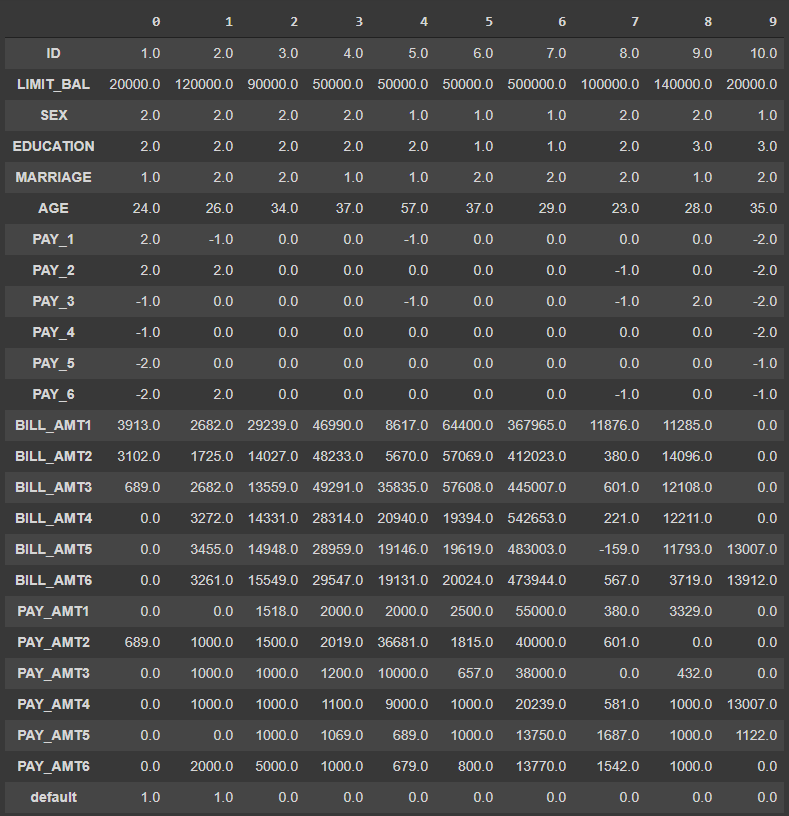
\includegraphics[width=5.21in,height=5.39in]{./media/image6.png}
	\end{Center}
\end{figure}


%%%%%%%%%%%%%%%%%%%% Figure/Image No: 2 Ends here %%%%%%%%%%%%%%%%%%%%


\vspace{\baselineskip}
\vspace{\baselineskip}

\vspace{\baselineskip}

\vspace{\baselineskip}

\vspace{\baselineskip}

\vspace{\baselineskip}

\vspace{\baselineskip}

\vspace{\baselineskip}
\section{Análisis 1D y 2D de datos}
\subsection{1D}
\textbf{Imagen 2.}
En esta segunda imagen generamos una tabla con las estadísticas unidimensionales, entre las cuales se encuentra:
\begin{itemize}
	\item La media
	\item La desviación estándar
	\item El valor mínimo de cada columna
	\item El cuartil q1(25$\%$ ), q2(50$\%$ ), q3(75$\%$ )
	\item El valor máximo de cada columna
\end{itemize}

\vspace{\baselineskip}


%%%%%%%%%%%%%%%%%%%% Figure/Image No: 3 starts here %%%%%%%%%%%%%%%%%%%%

\begin{figure}[H]
	\begin{Center}
		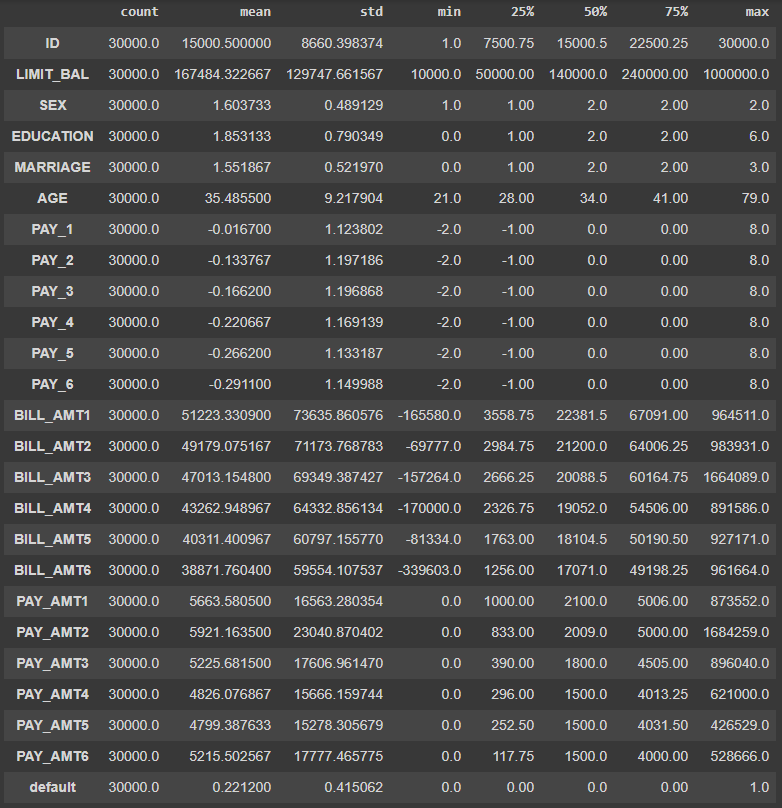
\includegraphics[width=5.86in,height=6.04in]{./media/image1.png}
	\end{Center}
\end{figure}


%%%%%%%%%%%%%%%%%%%% Figure/Image No: 3 Ends here %%%%%%%%%%%%%%%%%%%%

Con estos datos se puede armar una idea de que tan dispersos están los datos.

\vspace{\baselineskip}
\begin{justify}
\textbf{Imagen 3.}
\end{justify}
\begin{justify}
En esta imagen se hizo un gráfico de barras para visualizar el nivel de educación máximo que alcanzaron las personas del banco en Taiwán. De esta manera podremos identificar el nivel de educación que más predomina en el dataset.
\end{justify}
\begin{justify}
Para este caso aproximadamente 14.000 personas tienen como nivel educacional máximo la universidad, por lo que la mayoría de las personas solamente hizo el pregrado.
\end{justify}


%%%%%%%%%%%%%%%%%%%% Figure/Image No: 4 starts here %%%%%%%%%%%%%%%%%%%%

\begin{figure}[H]
	\begin{Center}
		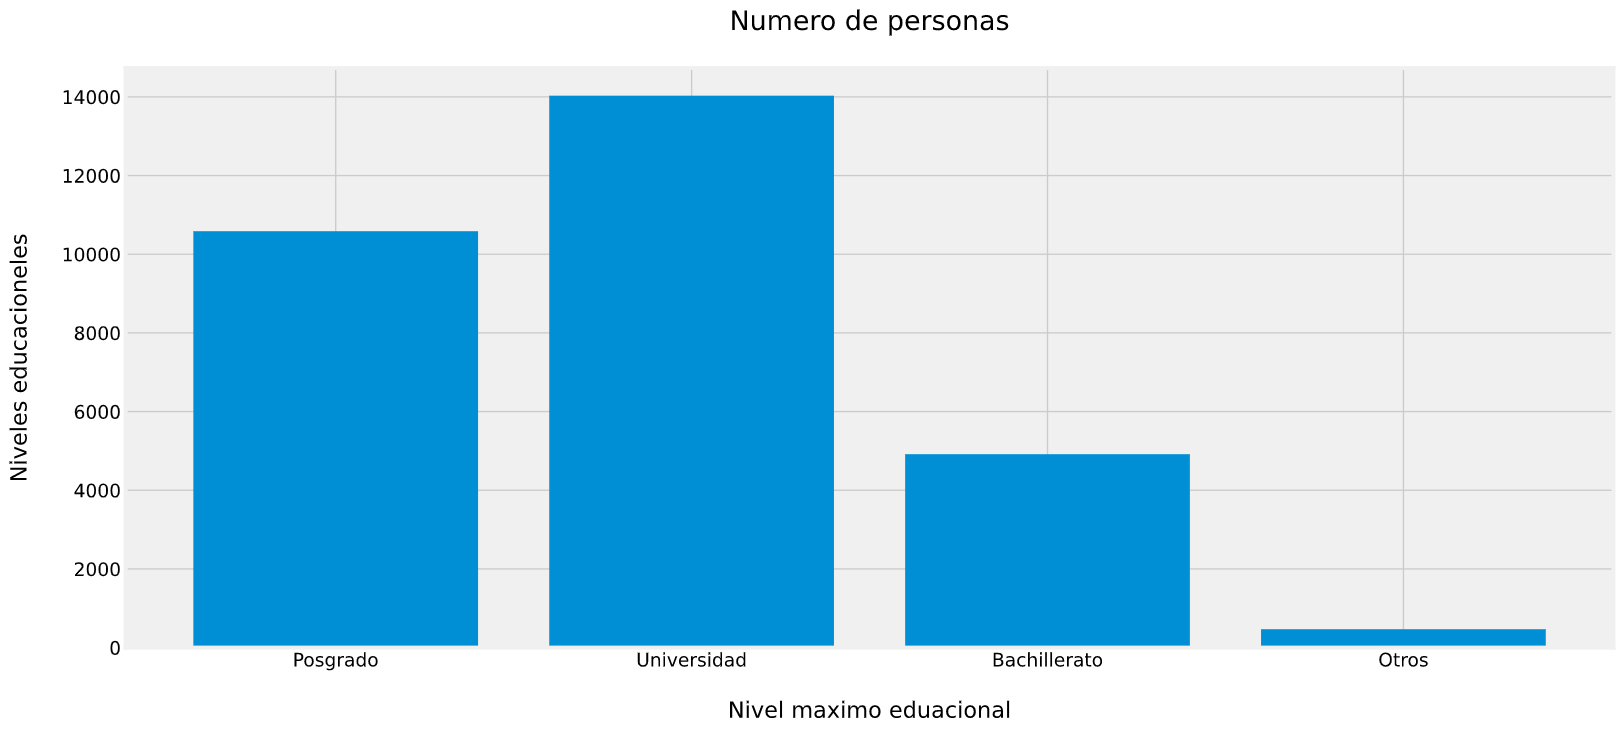
\includegraphics[width=6.27in,height=2.83in]{./media/image3.png}
	\end{Center}
\end{figure}


%%%%%%%%%%%%%%%%%%%% Figure/Image No: 4 Ends here %%%%%%%%%%%%%%%%%%%%


\vspace{\baselineskip}
\vspace{\baselineskip}
\begin{justify}
\textbf{Imagen 4.}
\end{justify}
\begin{justify}
En esta imagen hicimos un gráfico de barras para visualizar el estado civil de las personas del banco en Taiwán.
\end{justify}
\begin{justify}
Como resultado se obtuvo aproximadamente 16.000 personas solteras, por lo tanto podemos concluir que hay una cantidad considerable de personas solteras dentro del dataset.
\end{justify}


%%%%%%%%%%%%%%%%%%%% Figure/Image No: 5 starts here %%%%%%%%%%%%%%%%%%%%

\begin{figure}[H]
	\begin{Center}
		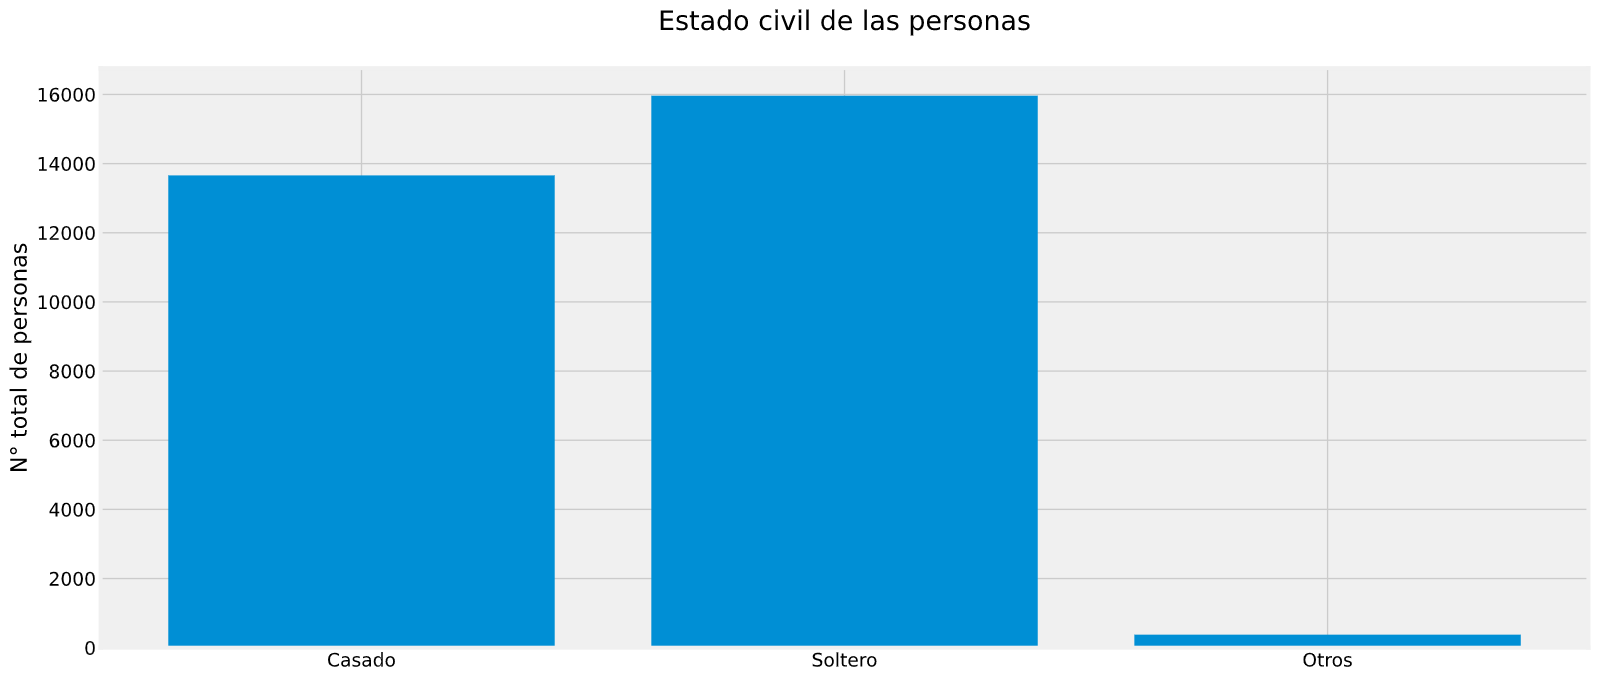
\includegraphics[width=6.27in,height=2.67in]{./media/image8.png}
	\end{Center}
\end{figure}


%%%%%%%%%%%%%%%%%%%% Figure/Image No: 5 Ends here %%%%%%%%%%%%%%%%%%%%


\vspace{\baselineskip}
\vspace{\baselineskip}
\begin{justify}
\textbf{Imagen 5.}
\end{justify}
\begin{justify}
En esta imagen hicimos un gráfico de barras para visualizar cuál es el sexo que mas predomina el el dataset.
\end{justify}
\begin{justify}
Claramente se visualiza que la mayoría de las personas en el dataset pertenecen al sexo femenino con mas de 17.500 personas.
\end{justify}


%%%%%%%%%%%%%%%%%%%% Figure/Image No: 6 starts here %%%%%%%%%%%%%%%%%%%%

\begin{figure}[H]
	\begin{Center}
		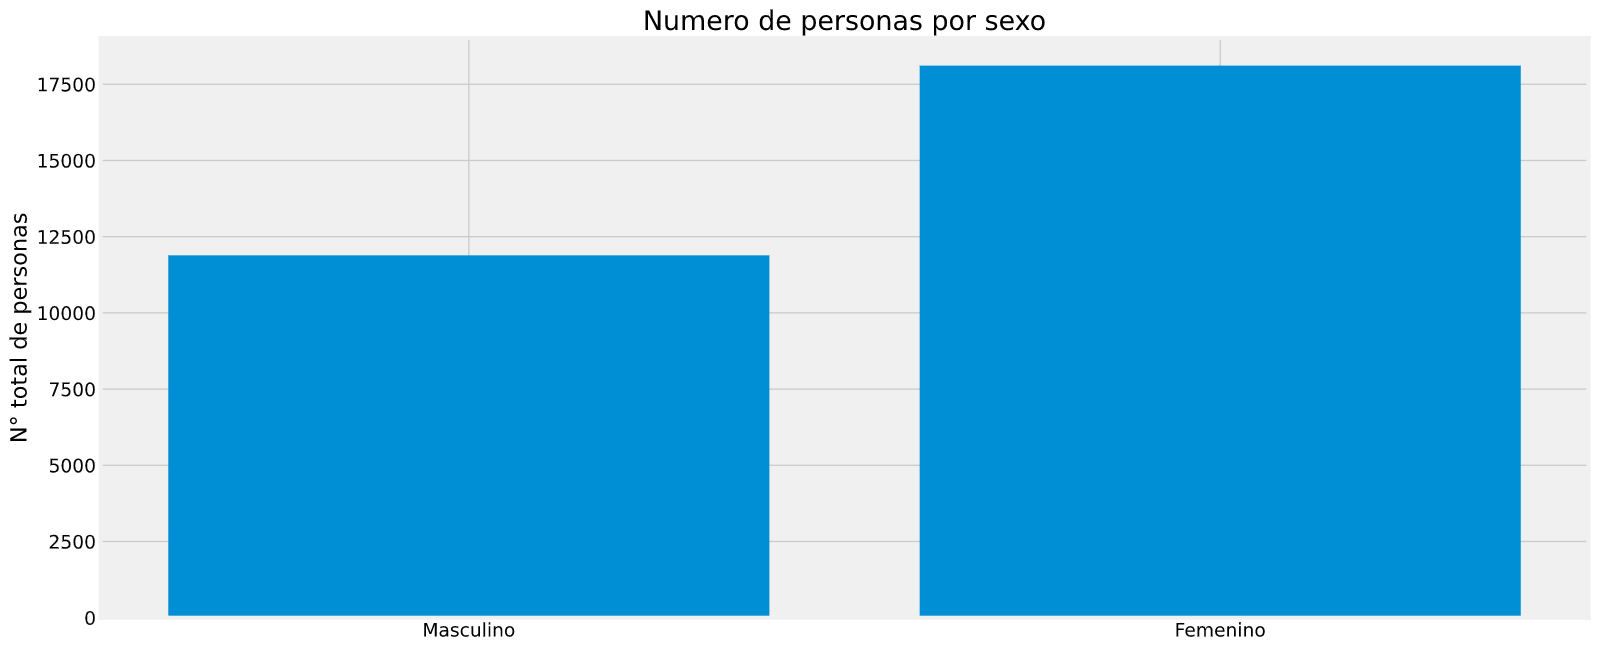
\includegraphics[width=6.27in,height=2.56in]{./media/image2.png}
	\end{Center}
\end{figure}


%%%%%%%%%%%%%%%%%%%% Figure/Image No: 6 Ends here %%%%%%%%%%%%%%%%%%%%


\vspace{\baselineskip}
\vspace{\baselineskip}
\begin{justify}
\textbf{Imagen 6.}
\end{justify}
\begin{justify}
En esta imagen hicimos un gráfico para visualizar la distribución de las edades en el dataset.
\end{justify}
\begin{justify}
Si\ hiciéramos una agrupación de edades en un rango de 5 años. tendríamos que la mayoría de los clientes del banco de Taiwán están entre los 25 y 30 años de edad, incluso la mediana es de  34 años.
\end{justify}


%%%%%%%%%%%%%%%%%%%% Figure/Image No: 7 starts here %%%%%%%%%%%%%%%%%%%%

\begin{figure}[H]
	\begin{Center}
		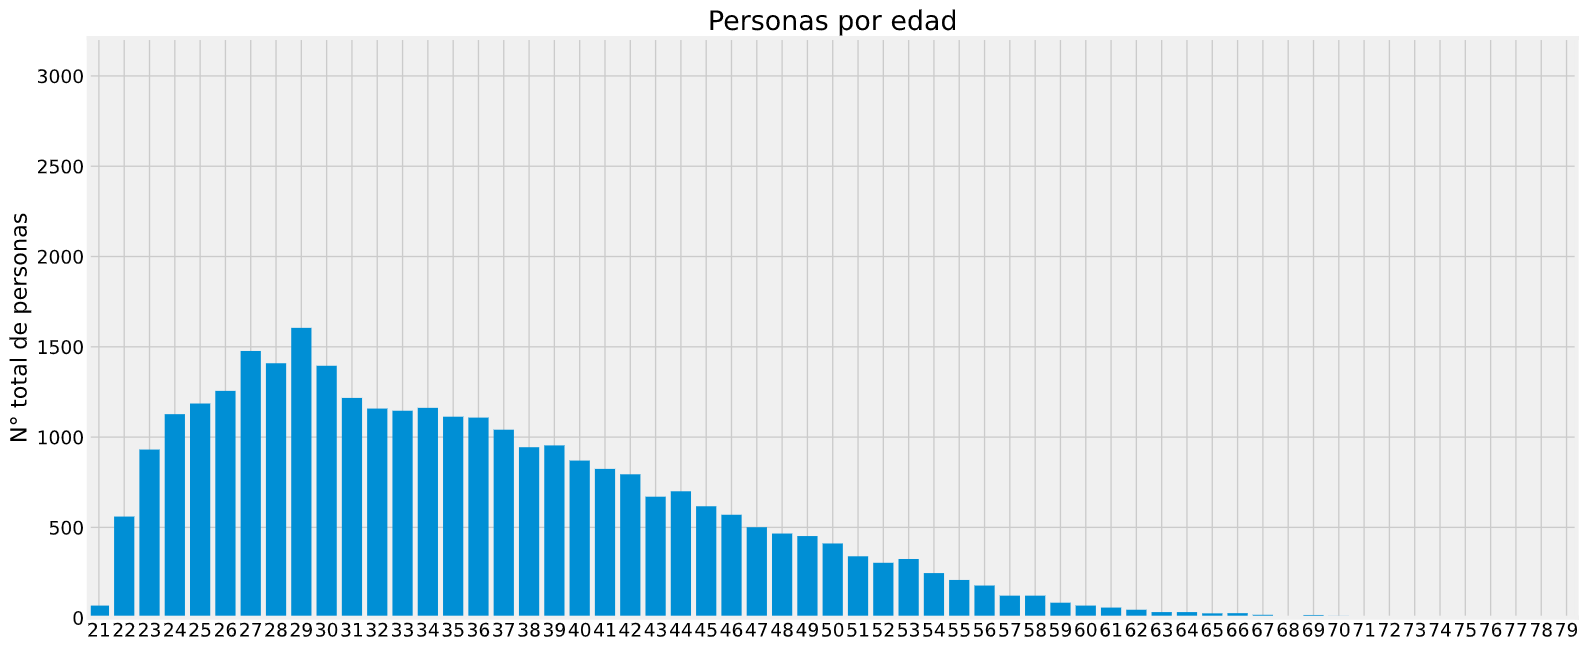
\includegraphics[width=6.27in,height=2.57in]{./media/image5.png}
	\end{Center}
\end{figure}


%%%%%%%%%%%%%%%%%%%% Figure/Image No: 7 Ends here %%%%%%%%%%%%%%%%%%%%


\vspace{\baselineskip}\subsection{2D}
\begin{justify}
\textbf{Imagen 7.}
\end{justify}
\begin{justify}
En esta imagen hicimos un gráfico Heatmap para visualizar la correlación entre las variables del dataset.
\end{justify}
\begin{justify}
El objetivo es encontrar las variables que tengan relación lineal entre ellas o aquellas que tengan una relación lineal inversa.
\end{justify}


%%%%%%%%%%%%%%%%%%%% Figure/Image No: 8 starts here %%%%%%%%%%%%%%%%%%%%

\begin{figure}[H]
	\begin{Center}
		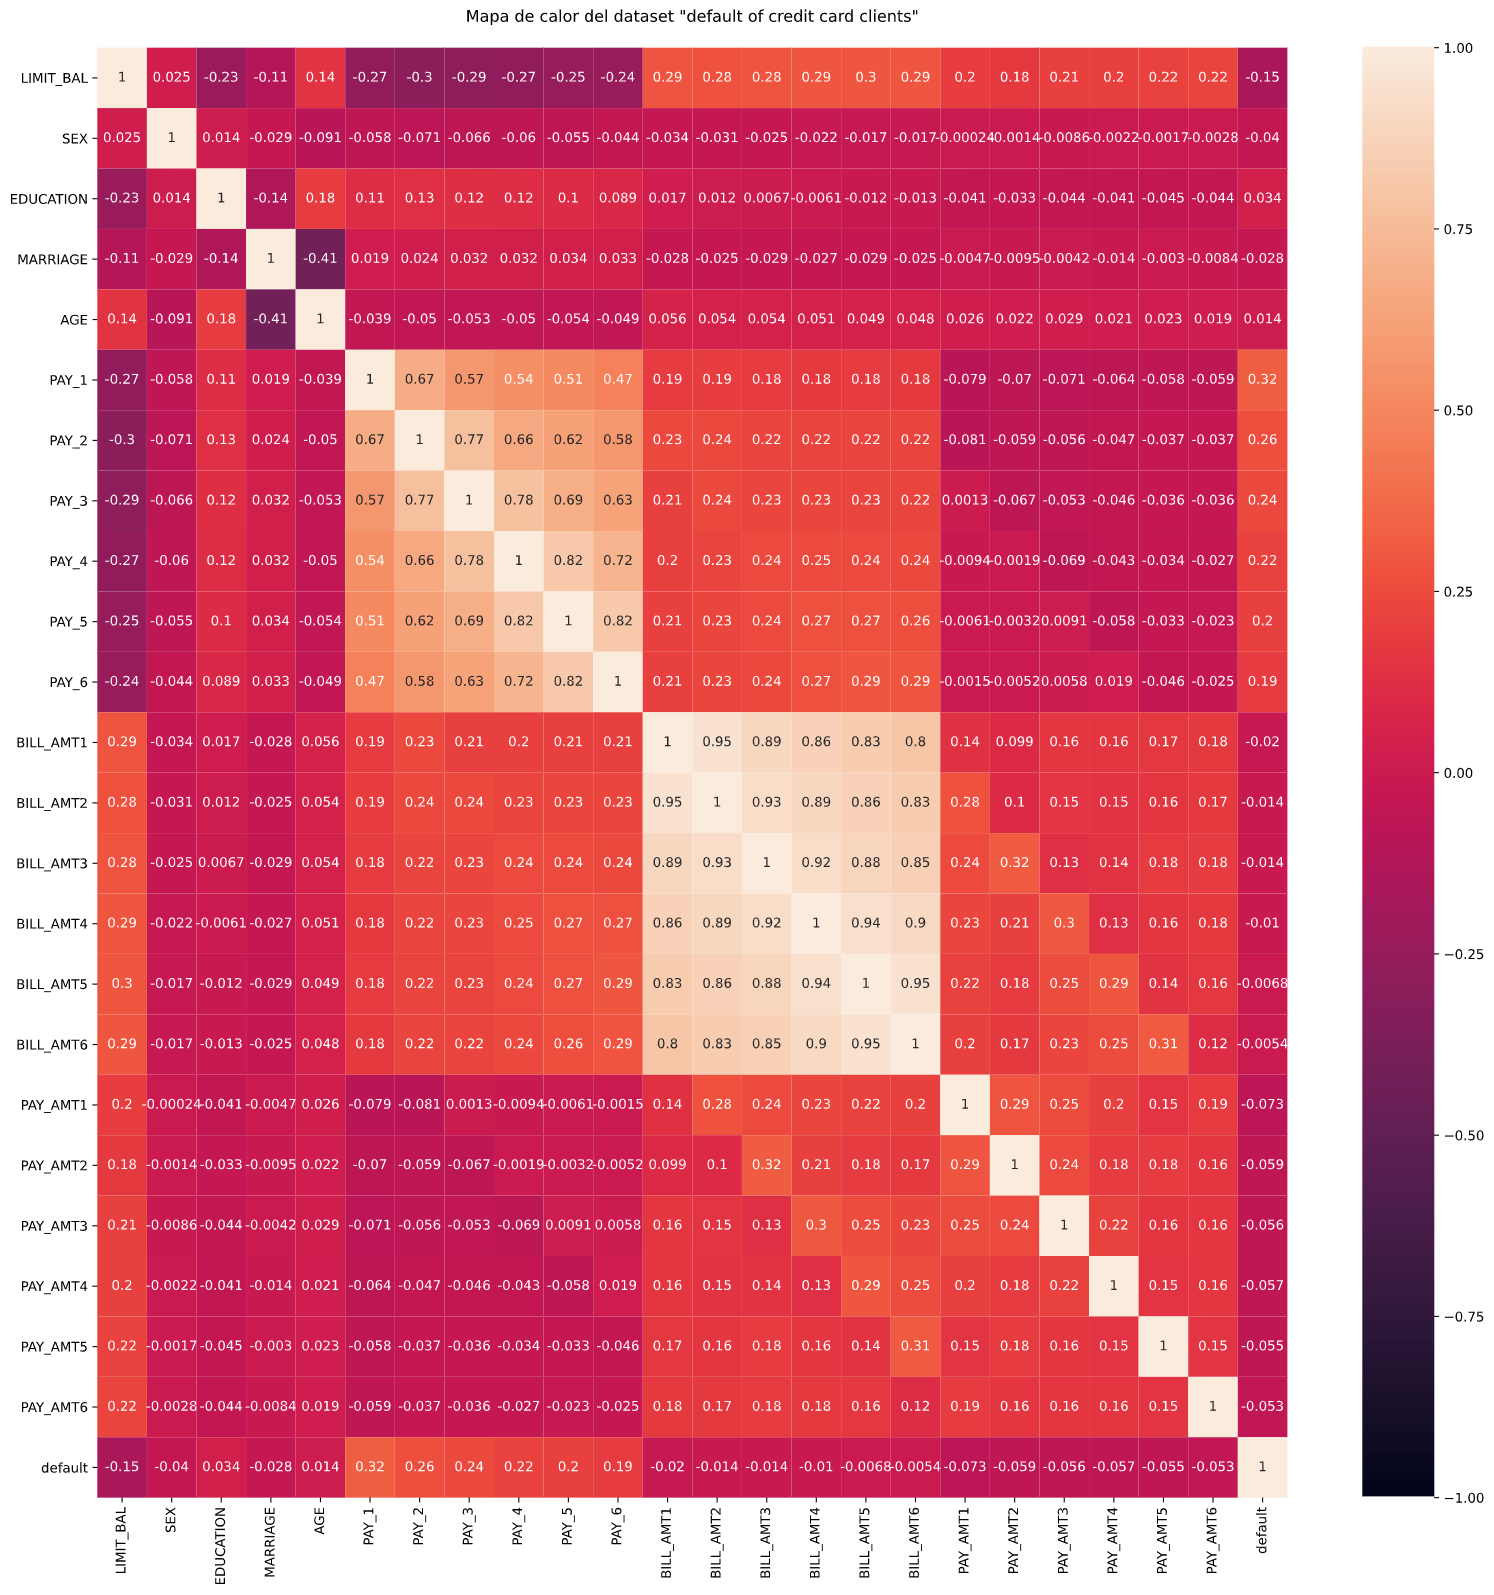
\includegraphics[width=6.27in,height=6.69in]{./media/image9.png}
	\end{Center}
\end{figure}


%%%%%%%%%%%%%%%%%%%% Figure/Image No: 8 Ends here %%%%%%%%%%%%%%%%%%%%


\vspace{\baselineskip}
\vspace{\baselineskip}
\vspace{\baselineskip}
\vspace{\baselineskip}
\vspace{\baselineskip}
\vspace{\baselineskip}
\vspace{\baselineskip}
\vspace{\baselineskip}
\begin{justify}
\textbf{Imagen 8.}
\end{justify}
\begin{justify}
En esta imagen hicimos un diagrama de dispersión entre el monto del crédito otorgado y el estado de la cuenta.
\end{justify}
\begin{justify}
En el Heatmap vimos que estas variables tenían un coeficiente de correlación de 0.3 aproximadamente, por lo que se puede decir que existe una relación leve entre estas.
\end{justify}


%%%%%%%%%%%%%%%%%%%% Figure/Image No: 9 starts here %%%%%%%%%%%%%%%%%%%%

\begin{figure}[H]
	\begin{Center}
		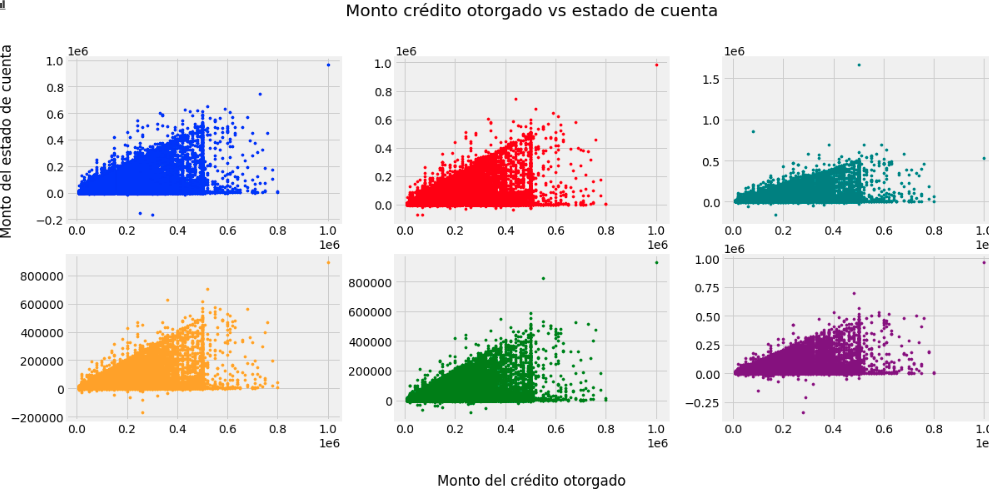
\includegraphics[width=6.27in,height=3.15in]{./media/image11.png}
	\end{Center}
\end{figure}


%%%%%%%%%%%%%%%%%%%% Figure/Image No: 9 Ends here %%%%%%%%%%%%%%%%%%%%


\vspace{\baselineskip}
\vspace{\baselineskip}

\vspace{\baselineskip}

\vspace{\baselineskip}

\vspace{\baselineskip}

\vspace{\baselineskip}

\vspace{\baselineskip}

\vspace{\baselineskip}

\vspace{\baselineskip}

\vspace{\baselineskip}

\vspace{\baselineskip}

\vspace{\baselineskip}

\vspace{\baselineskip}

\vspace{\baselineskip}

\vspace{\baselineskip}

\vspace{\baselineskip}

\vspace{\baselineskip}

\vspace{\baselineskip}

\vspace{\baselineskip}

\vspace{\baselineskip}

\vspace{\baselineskip}

\vspace{\baselineskip}

\vspace{\baselineskip}

\vspace{\baselineskip}

\vspace{\baselineskip}

\vspace{\baselineskip}

\vspace{\baselineskip}

\vspace{\baselineskip}

\vspace{\baselineskip}
\section{Preprocesamiento de datos}

\vspace{\baselineskip}
Se parte bajo la condición que no existen valores nulos dentro del data set.
Tampoco hay valores faltantes, cada columna tiene sus respectivos 30000 datos.

\vspace{\baselineskip}


%%%%%%%%%%%%%%%%%%%% Figure/Image No: 10 starts here %%%%%%%%%%%%%%%%%%%%

\begin{figure}[H]
	\begin{Center}
		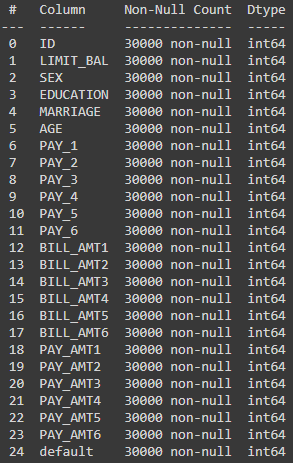
\includegraphics[width=3.05in,height=4.82in]{./media/image4.png}
	\end{Center}
\end{figure}


%%%%%%%%%%%%%%%%%%%% Figure/Image No: 10 Ends here %%%%%%%%%%%%%%%%%%%%


\vspace{\baselineskip}
\vspace{\baselineskip}

\vspace{\baselineskip}
ID: se eliminó esta columna.
Educación: se tomó los valores que no eran parte de las categorías(0, 5 y 6) según la documentación y se cambió por 4(otros).
Estado civil: se cambió los valores que no pertenecen a las categorías definidas en la documentación (0 en este caso) y se cambió por 3. 
Sexo: no fue necesario hacer un preprocesamiento adicional 

\vspace{\baselineskip}
Las decisiones que se tomaron fue considerando que las variables tenían dentro de sus categorías una variable $``$otros$"$  por lo tanto los datos no pertenecientes a las categorías documentadas podrían ser asignadas a dicha categoría, además los datos no categorizados dentro de las variables era muy bajo con respecto al conjunto total de datos por su respectiva columna, es más la variable educación tenía dentro de sus datos solo un 1.15$\%$  de datos no categorizados según documentación.
Otras posibles soluciones con respecto al preprocesamiento de los datos pudo haber sido la eliminación de las tuplas completas en donde alguna de sus columnas no estaban bien categorizadas o reemplazar dichos valores por la media de la columna debido a que esos valores no categorizados no eran los suficientes para afectar considerablemente la media o la mediana.

\vspace{\baselineskip}
\section{Diseño de experimentos}
Se\ considero el experimento de relacionar 2 variables las cuales aparentemente tenían una correlación bastantante fuerte, las cuales no podrían ayudar a nuestros algoritmos a  predecir con mayor exactitud
en\ los cuales se encontró un patrón entre  el estado de cuenta del mes siguiente y el monto del pago anterior.

\vspace{\baselineskip}


%%%%%%%%%%%%%%%%%%%% Figure/Image No: 11 starts here %%%%%%%%%%%%%%%%%%%%

\begin{figure}[H]
	\begin{Center}
		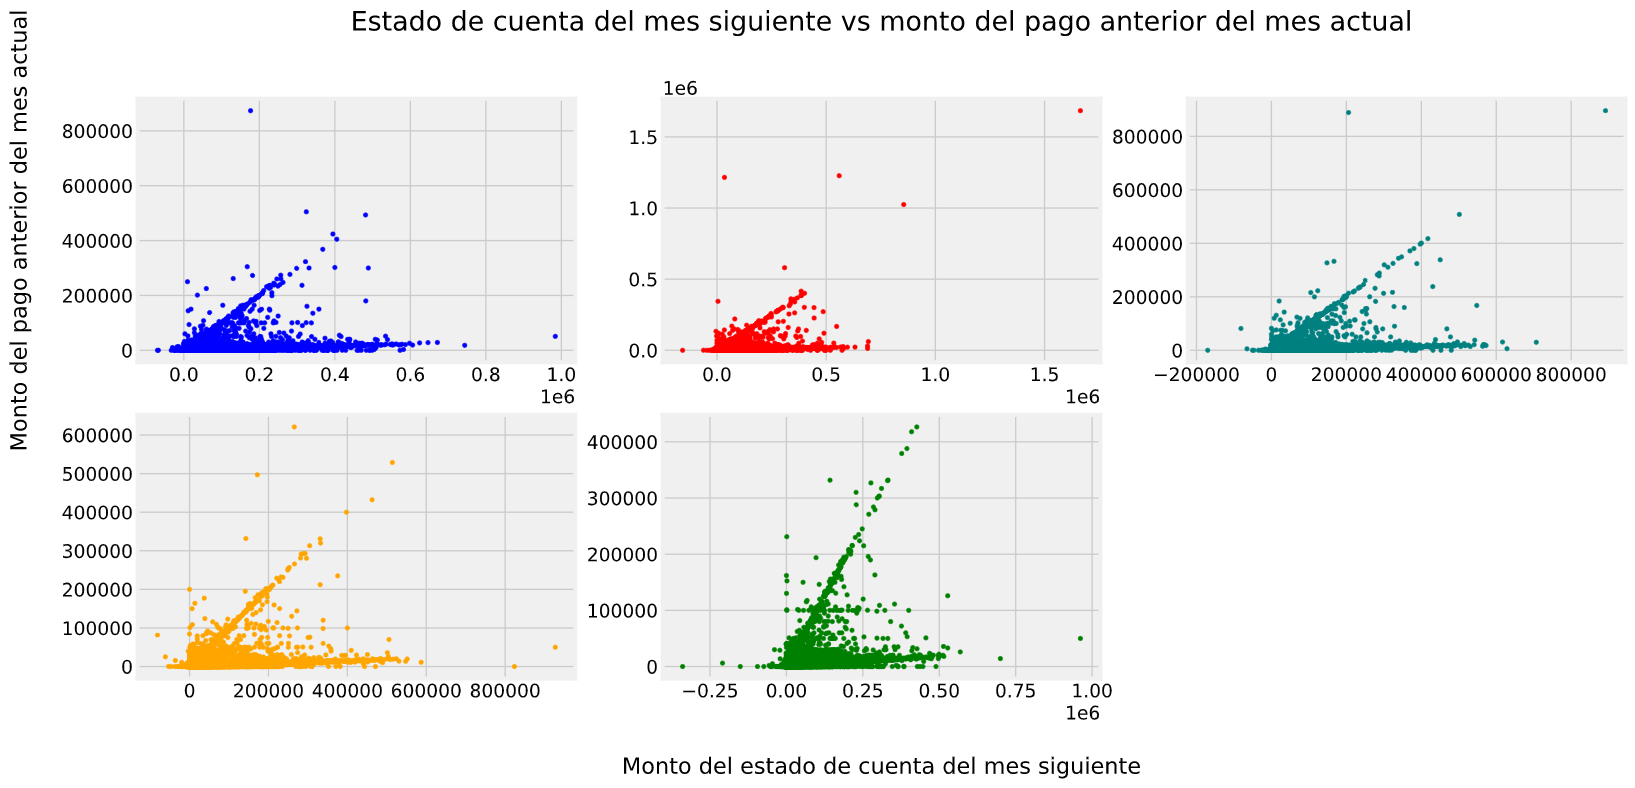
\includegraphics[width=6.27in,height=3.01in]{./media/image10.png}
	\end{Center}
\end{figure}


%%%%%%%%%%%%%%%%%%%% Figure/Image No: 11 Ends here %%%%%%%%%%%%%%%%%%%%


\vspace{\baselineskip} 

\vspace{\baselineskip}

\vspace{\baselineskip}

\vspace{\baselineskip}

\vspace{\baselineskip}

\vspace{\baselineskip}

\vspace{\baselineskip}

\vspace{\baselineskip}

\vspace{\baselineskip}

\vspace{\baselineskip}

\vspace{\baselineskip}

\vspace{\baselineskip}

\vspace{\baselineskip}

\vspace{\baselineskip}

\vspace{\baselineskip}
\section{Revisión métodos relacionados}

\vspace{\baselineskip}
\subsection{Primero}
Predictive Analysis of Credit Score for Credit Card Defaulters
Nupura Torvekar, Pravin S. Game - Enero 2019

\vspace{\baselineskip}
\href{https://www.researchgate.net/profile/Pravin-Game/publication/332557433_Predictive_analysis_of_credit_score_for_credit_card_defaulters/links/5f44ec63458515b7294fc74c/Predictive-analysis-of-credit-score-for-credit-card-defaulters.pdf}{\textcolor[HTML]{1155CC}{\ul{https://www.researchgate.net/profile/Pravin-Game/publication/332557433\_Predictive\_analysis\_of\_credit\_score\_for\_credit\_card\_defaulters/links/5f44ec63458515b7294fc74c/Predictive-analysis-of-credit-score-for-credit-card-defaulters.pdf}}}

\vspace{\baselineskip}
Que proponen: 

\vspace{\baselineskip}
Los\ autores le dan énfasis al contexto en el que se encuentra el sector bancario afirmando que  es uno de los más volátiles y vulnerables en el mundo con sus factores de riesgo cada vez mayores.
El\ riesgo de crédito continúa siendo un factor integral para que las instituciones bancarias  sufran pérdidas del orden de cientos de millones de dólares debido a la imposibilidad de recuperar el dinero concedido a los clientes.

\vspace{\baselineskip}
Que utilizaron:

\vspace{\baselineskip}
Naive Bayes, Regresión logística, máquinas de vectores de soporte y bosque aleatorio. Los algoritmos anteriores se evalúan utilizando entorno weka para aprendizaje automático y la minería de datos, además se usa KNIME que es una plataforma de minería de datos que permite el desarrollo de modelos en un entorno visual.

\vspace{\baselineskip}
Que encontraron:

\vspace{\baselineskip}
Los autores afirman que el uso de técnicas de aprendizaje automático para la predicción de los morosos de tarjetas de crédito es esencial para la identificación de riesgo crediticio. Esto puede ayudar a las instituciones financieras a diseñar sus estrategias futuras.
En cuanto a los algoritmos utilizados los autores evaluaron los clasificadores utilizando la precisión de su predicción. Encontraron que el clasificador con la mayor precisión es el bosque aleatorio.

\vspace{\baselineskip}

\vspace{\baselineskip}

\vspace{\baselineskip}

\vspace{\baselineskip}

\vspace{\baselineskip}
\subsection{Segundo}
Machine Learning Approaches to Predict Default of Credit Card Clients
{\fontsize{10pt}{12.0pt}\selectfont Ruilin Liu - 2018.}
\href{https://www.scirp.org/html/7-7201927_88577.htm?pagespeed=noscript}{\textcolor[HTML]{1155CC}{\ul{https://www.scirp.org/html/7-7201927\_88577.htm?pagespeed=noscript}}}

\vspace{\baselineskip}
Que proponen: 
El autor afirma que la red neuronal puede explorar la relación entre las características de entrada y las etiquetas correspondientes, por lo que es adecuada para problemas complejos de aprendizaje automático. Por otro lado, otros modelos de aprendizaje automático como la regresión lineal o máquinas vectores de soporte pueden resolver problemas más simples de manera más eficiente. Por tanto, después de analizar problemas específicos, se debe responder a la pregunta de $``$¿es realmente necesaria la red neuronal en este caso?Además el autor menciona que existen varios tipos de redes neuronales.

\vspace{\baselineskip}
Que utilizaron:
El autor utiliza varios modelos entre ellos k-vecinos cercanos, máquinas vector de soporte, árbol de decisión, bosques aleatorios, redes neuronales y redes neuronales recurrentes.

\vspace{\baselineskip}

\vspace{\baselineskip}
Que encontraron:
El autor afirma que los modelos tradicionales de aprendizaje automático solo pueden lograr una precisión de 0,8040, que se logra con SVM es decir mayor a los demás. La mayor precisión de la red neuronal es 0,8246, por lo tanto el autor concluye que las redes neuronales superan a los modelos tradicionales, excepto en situaciones en las que la investigación se centra fuertemente en predicciones positivas.

\vspace{\baselineskip}
\subsection{Tercero}
Real Time Credit Card Default Classification Using Adaptive Boosting-Based Online Learning Algorithm
Hongya Lu, Haifeng Wang and Sang Won Yoon Department of Systems Science and Industrial Engineering State University of New York at Binghamton, Binghamton, NY- 2017

\vspace{\baselineskip}
\href{https://www.researchgate.net/profile/Haifeng-Wang-25/publication/319689046_Real_Time_Credit_Card_Default_Classification_Using_Adaptive_Boosting-Based_Online_Learning_Algorithm/links/59b991e1458515bb9c48a3f8/Real-Time-Credit-Card-Default-Classification-Using-Adaptive-Boosting-Based-Online-Learning-Algorithm.pdf}{\textcolor[HTML]{1155CC}{\ul{https://www.researchgate.net/profile/Haifeng-Wang-25/publication/319689046\_Real\_Time\_Credit\_Card\_Default\_Classification\_Using\_Adaptive\_Boosting-Based\_Online\_Learning\_Algorithm/links/59b991e1458515bb9c48a3f8/Real-Time-Credit-Card-Default-Classification-Using-Adaptive-Boosting-Based-Online-Learning-Algorithm.pdf}}}

\vspace{\baselineskip}
Que proponen: 
Los\ investigadores\  proponen una aplicación de aprendizaje en línea al sistema de detección de incumplimiento de tarjetas de crédito que logra un ajuste del modelo en tiempo real con un mínimo esfuerzo computacional. Para los emisores de tarjetas de crédito, el número de clientes de tarjetas de crédito, la  cantidad de consumo y las tasas de incumplimiento son factores que influyen en la participación de los bancos en el mercado. Los autores además afirman que el banco sufrirá pérdidas debido a una mala gestión de la administración de tarjetas de créditos.

\vspace{\baselineskip}

\vspace{\baselineskip}
Que utilizaron:
Los autores utilizaron una técnica que se llama aprendizaje. Los investigadores explican que el aprendizaje en línea representa una familia de algoritmos eficientes y escalables en comparación con el aprendizaje por lotes tradicional, y aborda los problemas de la memoria.
costes de consumo y reciclaje con nuevos datos entrantes.
Las técnicas exactas que utilizan los investigadores son métodos de máquina de aprendizaje extremo secuencial en línea (OS-ELM) y aumento de adaptación secuencial en línea (OS-AdaBoost). El OS-ELM está adaptado de la Extreme Learning Machine básica
(ELM) para permitir que el modelo aprenda uno a uno fragmento a fragmento . El ELM básico propone una red feedforward con una única capa oculta generalizada que no funciona estrictamente como neuronas.

\vspace{\baselineskip}
Que encontraron:
Los autores mencionan que con las técnicas en línea a otras técnicas con determinadas medidas de rendimiento, se obtienen resultados experimentales en comparación a modelos tradicionales de aprendizaje automático, además los autores afirman que el aprendizaje en línea tiene un gran potencial para los problemas de identificación en tiempo real y que esa idea genera futuras discusiones y un gran potencial investigativo.

\vspace{\baselineskip}

\vspace{\baselineskip}
\subsection{Cuarto}
Estimation of Credit Card Customers Payment Status by Using kNN and MLP
Murat KOKLU, Kadir SABANCI - 2016
\href{https://www.ijisae.org/IJISAE/article/view/969/546}{\textcolor[HTML]{1155CC}{\ul{https://www.ijisae.org/IJISAE/article/view/969/546}}}

\vspace{\baselineskip}
Que proponen: 
Los\ autores\ afirman\ que para los bancos, lo más importante durante la comercialización de tarjetas de crédito es la capacidad de pago de los clientes. Los investigadores en el estudio proponen una estimación del estado de pago para los clientes de tarjetas de crédito. Para ello  han utilizado algoritmos de minería de datos.  Los autores describen la minería de datos como  un proceso computacional que revela patrones en conjuntos de datos utilizando métodos como inteligencia artificial, aprendizaje automático, estadísticas, etc. Los métodos utilizados en la minería de datos se investigan en dos grupos: predictivos y descriptivos

\vspace{\baselineskip}
Que utilizaron:
Los\ autores utilizaron entorno Weka  para el análisis de aprendizaje automático y recurrieron al uso de modelos predictivos como {\fontsize{11pt}{13.2pt}\selectfont k-nn, mlp( percepción multicapa)}

\vspace{\baselineskip}
Que encontraron:
Utilizando\ el algoritmo knn, los autores obtuvieron  tasas de éxito de la estimación de pago para diferentes valores de k. Se han alcanzado el error medio absoluto (MAE) y el error cuadrático medio (RMSE), el éxito de la estimación del método k-nn (en porcentaje), además en el estudio mencionan el impacto basado en MAE y RMSE según cuantos k vecinos se elija.

\vspace{\baselineskip}

\vspace{\baselineskip}

\vspace{\baselineskip}

\vspace{\baselineskip}

\vspace{\baselineskip}

\vspace{\baselineskip}

\vspace{\baselineskip}

\vspace{\baselineskip}

\vspace{\baselineskip}

\vspace{\baselineskip}

\vspace{\baselineskip}

\vspace{\baselineskip}

\vspace{\baselineskip}

\vspace{\baselineskip}

\vspace{\baselineskip}

\vspace{\baselineskip}

\vspace{\baselineskip}

\vspace{\baselineskip}

\vspace{\baselineskip}

\vspace{\baselineskip}

\vspace{\baselineskip}

\vspace{\baselineskip}

\vspace{\baselineskip}

\vspace{\baselineskip}

\vspace{\baselineskip}

\vspace{\baselineskip}

\vspace{\baselineskip}

\vspace{\baselineskip}

\vspace{\baselineskip}

\vspace{\baselineskip}

\vspace{\baselineskip}

\vspace{\baselineskip}

\vspace{\baselineskip}

\vspace{\baselineskip}
\section{Descripción de algoritmos básicos}

\vspace{\baselineskip}

\vspace{\baselineskip}

\vspace{\baselineskip}
\subsection{Árbol de decisión}
Es un modelo analítico que a través de una representación esquemática de las alternativas disponible facilita la toma de mejores decisiones para obtener un resultado. Su nombre deriva de la apariencia del modelo parecido a un árbol y su uso es amplio en el ámbito de la toma de decisiones bajo incertidumbre (Teoría de Decisiones).
Este modelo sirve para resolver problemas de clasificación.

\vspace{\baselineskip}
La división entre valores de entrenamiento se hizo utilizando la técnica hold-out separando 30 test y 70 de entrenamiento.
En el problema que se busca solucionar se utilizó como criterio la entropía y de máxima profundidad un valor de 10.
\subsection{Naive Bayes}
En\ un sentido muy general, el modelo naive bayes es una clase especial de algoritmos de clasificación de Aprendizaje Automático el cual  se basan en el teorema de bayes.
En\ este tipo de modelo se asume que las variables predictoras son independientes entre sí. En otras palabras,  la presencia de una cierta característica en un conjunto de datos no está en absoluto relacionada con cualquier otra característica.

\vspace{\baselineskip}
La división entre valores de entrenamiento se hizo utilizando la técnica hold-out separando 20 test y 80 de entrenamiento.
Para implementar el algoritmo se usó como parámetro binarización de 0.5.

\vspace{\baselineskip}

\vspace{\baselineskip}

\vspace{\baselineskip}

\vspace{\baselineskip}

\vspace{\baselineskip}

\vspace{\baselineskip}
{\fontsize{20pt}{24.0pt}\selectfont \textbf{ }}

\vspace{\baselineskip}
\section{Reporte de resultados}
Después de que se hayan implementado ambos algoritmos el que obtuvo mejores resultados con una diferencia mínima y tomando en consideración el accuracy fue naive bayes con una métrica accuracy de 0.793 frente a la métrica del árbol de decisión que obtuvo 0.776.

\vspace{\baselineskip}

\vspace{\baselineskip}

\vspace{\baselineskip}

\vspace{\baselineskip}

\vspace{\baselineskip}

\vspace{\baselineskip}

\vspace{\baselineskip}

\vspace{\baselineskip}

\vspace{\baselineskip}

\vspace{\baselineskip}

\vspace{\baselineskip}

\vspace{\baselineskip}

\vspace{\baselineskip}

\vspace{\baselineskip}
\vspace{\baselineskip}
\vspace{\baselineskip}
\vspace{\baselineskip}
\vspace{\baselineskip}
\vspace{\baselineskip}
\vspace{\baselineskip}
\vspace{\baselineskip}
\vspace{\baselineskip}
\vspace{\baselineskip}
\vspace{\baselineskip}
\vspace{\baselineskip}
\vspace{\baselineskip}
\vspace{\baselineskip}
\vspace{\baselineskip}

\vspace{\baselineskip}
\section{Conclusión}

\vspace{\baselineskip}
Finalmente podemos considerar que existen 3 posibles caminos si hablamos de preprocesamiento los cuales eran eliminar, reemplazar por media/mediana y re asignar los valores mal categorizados a la categoría que correspondan (otros).
En cuanto a las correlaciones que se pudieron encontrar en los diagramas 2D fueron el monto crédito otorgado vs el estado de cuenta donde existía una correlación positiva un tanto débil pero considerable, entre otras variables con relaciones interesantes. Cabe destacar que en esta primera etapa se puede evidenciar que existen relaciones entre las variables y que esto nos permitirá a futuro entrenar modelos predictivos de manera idónea.
Otro\ punto importante que podemos concluir en base a los paper mencionados en este trabajo, es que existen múltiples caminos para dar solución a este problema, algunos caminos  priorizan la eficiencia en función del tiempo para eventualmente poder implementar la solución en entornos de tiempo real, otras formas utilizan algoritmos más tradicionales los cuales prácticamente son un estándar cuando de clasificar hablamos, sin embargo el método que se considera como mejor solución actual en condiciones normales es el uso de redes neuronales en otras palabras deep learning, este método es catalogado como la mejor solución en dos de los cuatro paper, y en la página oficial de ics uci.
Actualmente el deep learning, nlp y la inteligencia artificial nos ha llevado a avanzar a pasos agigantados en múltiples problemas que anteriormente la solución no era la mejor o simplemente no era óptima.

\vspace{\baselineskip}

\vspace{\baselineskip}

\vspace{\baselineskip}

\vspace{\baselineskip}

\vspace{\baselineskip}

\vspace{\baselineskip}

\vspace{\baselineskip}

\vspace{\baselineskip}

\vspace{\baselineskip}

\vspace{\baselineskip}

\vspace{\baselineskip}

\vspace{\baselineskip}

\vspace{\baselineskip}

\vspace{\baselineskip}

\vspace{\baselineskip}

\vspace{\baselineskip}

\vspace{\baselineskip}

\vspace{\baselineskip}

\vspace{\baselineskip}

\vspace{\baselineskip}

\vspace{\baselineskip}

\vspace{\baselineskip}

\vspace{\baselineskip}
\section{Bibliografía }

\vspace{\baselineskip}

\vspace{\baselineskip}
\begin{itemize}
	\item \href{https://archive.ics.uci.edu/ml/datasets/default+of+credit+card+clients#}{\textcolor[HTML]{1155CC}{\ul{https://archive.ics.uci.edu/ml/datasets/default+of+credit+card+clients}}}
	\item \href{https://pandas.pydata.org/docs/}{\textcolor[HTML]{1155CC}{\ul{https://pandas.pydata.org/docs/}}}
	\item \href{https://matplotlib.org/stable/tutorials/introductory/pyplot.html#sphx-glr-tutorials-introductory-pyplot-py}{\textcolor[HTML]{1155CC}{\ul{https://matplotlib.org/stable/tutorials/introductory/pyplot.html$\#$ sphx-glr-tutorials-introductory-pyplot-py}}}
	\item \href{https://matplotlib.org/stable/gallery/images_contours_and_fields/image_annotated_heatmap.html}{\textcolor[HTML]{1155CC}{\ul{https://matplotlib.org/stable/gallery/images\_contours\_and\_fields/image\_annotated\_heatmap.html}}}

\vspace{\baselineskip}
	\item \href{https://www.researchgate.net/profile/Pravin-Game/publication/332557433_Predictive_analysis_of_credit_score_for_credit_card_defaulters/links/5f44ec63458515b7294fc74c/Predictive-analysis-of-credit-score-for-credit-card-defaulters.pdf}{\textcolor[HTML]{1155CC}{\ul{https://www.researchgate.net/profile/Pravin-Game/publication/332557433\_Predictive\_analysis\_of\_credit\_score\_for\_credit\_card\_defaulters/links/5f44ec63458515b7294fc74c/Predictive-analysis-of-credit-score-for-credit-card-defaulters.pdf}}}
	\item \href{https://www.ijisae.org/IJISAE/article/view/969/546}{\textcolor[HTML]{1155CC}{\ul{https://www.ijisae.org/IJISAE/article/view/969/546}}}
	\item \href{https://www.researchgate.net/profile/Haifeng-Wang-25/publication/319689046_Real_Time_Credit_Card_Default_Classification_Using_Adaptive_Boosting-Based_Online_Learning_Algorithm/links/59b991e1458515bb9c48a3f8/Real-Time-Credit-Card-Default-Classification-Using-Adaptive-Boosting-Based-Online-Learning-Algorithm.pdf}{\textcolor[HTML]{1155CC}{\ul{https://www.researchgate.net/profile/Haifeng-Wang-25/publication/319689046\_Real\_Time\_Credit\_Card\_Default\_Classification\_Using\_Adaptive\_Boosting-Based\_Online\_Learning\_Algorithm/links/59b991e1458515bb9c48a3f8/Real-Time-Credit-Card-Default-Classification-Using-Adaptive-Boosting-Based-Online-Learning-Algorithm.pdf}}}
	\item \href{https://www.scirp.org/html/7-7201927_88577.htm?pagespeed=noscript}{\textcolor[HTML]{1155CC}{\ul{https://www.scirp.org/html/7-7201927\_88577.htm?pagespeed=noscript}}}
	\item \href{https://scikit-learn.org/stable/modules/generated/sklearn.naive_bayes.BernoulliNB.html}{\textcolor[HTML]{1155CC}{\ul{https://scikit-learn.org/stable/modules/generated/sklearn.naive\_bayes.BernoulliNB.html}}}
	\item \href{https://scikit-learn.org/stable/modules/generated/sklearn.tree.DecisionTreeClassifier.html}{\textcolor[HTML]{1155CC}{\ul{https://scikit-learn.org/stable/modules/generated/sklearn.tree.DecisionTreeClassifier.html}}}
\end{itemize}

\vspace{\baselineskip}

\vspace{\baselineskip}

\vspace{\baselineskip}

\vspace{\baselineskip}

\vspace{\baselineskip}

\vspace{\baselineskip}

\vspace{\baselineskip}

\vspace{\baselineskip}
\printbibliography
\end{document}